\chapter{Éléments de méthodologie}

Le travail présenté dans cette thèse repose sur de travaux expérimentaux et
théoriques. En particulier, la partie expérimentale a été centrée sur l'étude de
populations de Collemboles de l'espèce \textit{Folsomia candida} élevée en
microcosmes au laboratoire. Dans ce chapitre, nous présenterons notre espèce
modèle du point de vu de sa biologie, de son intérêt pour les études menées, et
des conditions d'élevages. Puis nous détaillerons quelques développements
méthodologique qui ont permis l'accomplissement de nos travaux. 

\section{Le collembole, un modèle d'étude en écologie des populations}
\sectionmark{Le collembole modèle d'étude}

\subsection{Quelques généralités}

les Collemboles sont de petits arthropodes hexapodes entognathes aptères
mesurant généralement 1 à 5 mm. C'est un groupe très anciens qui compte
notamment l'un des plus vieux fossiles d'héxapode connu (\textit{Rhyniella
praecursor}). Aujourd'hui, plus de 8000 espèces ont été décrites
\autocites{bellinger2014a}, réparties dans l'ensemble des écosystèmes connus, en
faisant une des lignées d'arthropodes les plus communes au monde. Bien que
proches des Insectes, les Collemboles forment une classe à part, à côté des
Diploures, des Protoures et des Insectes \autocites{grimaldi2010a}. Ils sont
classés en quatre ordres: les Poduromorphes, les Entomobryomorphes, les
Symphypléones et les Néanuridés.

Les Collemboles se distinguent de leurs groupes frères par plusieurs
caractéristiques qui leur sont propres. En particulier, on note la présence
d'un organe de saut, la furca, à l'extrémité de l'abdomen. La furca est
habituellement repliée sous l'abdomen, retenue par le rétinacle. L'ouverture du
rétinacle relâche la furca, ce qui propulse le collembole sur plusieurs
centimètres. Certaines espèces de collemboles ont perdu secondairement cet
organe. On note également la présence d'un tube ventral, essentiel dans la
régulation de l'équilibre osmotique des individus.

Répandus dans l'ensemble des écosystèmes terrestres à toutes les latitudes, les
collemboles vivent généralement dans le sol où ils
peuvent atteindre des densité jusqu'à plusieurs dizaines de milliers d'individus
par $m^2$. Il se nourrissent principalement de déchets organiques présents dans
la litière, ou d'hyphes de champignons, et participent ainsi au recyclage de la
matière organique.

Les collemboles sont amétaboles et sont caractérisés par un développement direct
et une reproduction itéropare. Les juvéniles sont semblables aux adultes. De
parts leur mode de respiration cuticulaire, ils sont extrêmement sensibles à
l'humidité relative de leur environnement, et se regroupent généralement dans
les microcosmes les plus humides de leur habitat. 

\subsection{Le Collembole \textit{Folsomia candida}}

\subsubsection{Présentation}

\begin{figure}[!ht]
\begin{center}
\includegraphics[width=3cm,angle=90]{1_CorpsDeThese/Methodo/folsomiacandida.pdf}
\caption[\lofimage{1_CorpsDeThese/Methodo/folsomiacandida.pdf} Collembole
\textit{Folsomia candida}]{Collembole
\textit{Folsomia candida}}
\label{fig:folsomia}
\end{center}
\end{figure}


\textit{Folsomia candida} est un représentant très commun des Collemboles
(Figure \ref{fig:folsomia}), que l'on retrouve dans le monde entier. Il s'agit d'un
Collembole \textit{Arthropléone} de la superfamille des \textit{Entomobryoidae} et de la
famille des \textit{Isotomidae}. Cette famille comprend plus de 1000 espèces.
Une des caractéristiques principales de la famille des \textit{Isotomidae} est
que les segments abdominaux sont de même taille, contrairement aux autres
familles où le 4ème segment est généralement plus grand. 

\textit{Folsomia candida} vit principalement dans les couches profondes du sol
(euedaphique) et quelques fois dans des caves ou des grottes. Il est très
répandu mais difficile à observé car extrêmement sensible à la dessiccation. On
le retrouve couramment dans des bois morts en phase avancée de décomposition
dans un sol humide. C'est une espèce petite ($\approx 1 - 2 mm$) aveugle et
blanche qu'il est aisé de maintenir en laboratoire dans des boites de petites
dimension. 

\subsubsection{Mode de reproduction}

La grande majorité des populations de collembole \textit{Folsomia candida} est
composé exclusivement de femelles dont la reproduction est parthénogénétique.
Cependant, certaines populations possèdent des mâles rares avec une reproduction
sexuelle facultative, et d'autre sont encore strictement sexuées. Chez
\textit{Folsomia candida} la parthénogénèse est possible grâce à l'infection par
la bactérie \textit{Wolbachia} qui permet vraisemblablement la duplication de
l'ADN dans l'oeuf sans division cellulaire, et ainsi à l'oeuf de passer d'un
état haploïde à un état diploïde sans fécondation. 

Ce mode de reproduction conduit à des lignées génétiques distinctes dont les
trajectoires évolutives sont diversifiées, conduisant aujourd'hui à des
populations aux stratégies d'histoires de vie parfois contrastés
\autocites{tully2004a,tully2008a}. Dans ces travaux de thèse,
\textcites{tully2004a} a réalisé une classification de 11 lignées clonales
issues de zones géographiques différentes. Cette classification a permis de
distinguer deux clades dont les stratégies d'histoires de vie sont très variées.
Au cours de cette thèse, nous nous sommes intéressés à deux lignées génétiques
issus chacun d'un clade différent, ``HA'' et ``TO''. Ces deux lignées nous
permettent de comparer les réponses à la compétition par interférence et à la
température de populations aux stratégies biodémographiques contrastées.

\subsubsection{Croissance et reproduction continues}

Comparée à d'autres espèces couramment utilisées, \textit{Folsomia candida}
présente plusieurs avantages en tant qu'espèce modèle en écologie, en
particulier lorsque l'on s'intéresse aux traits d'histoire de vie comme la
taille corporelle qui détermine la dynamique de la structure de la population.
Les collemboles de cette espèce se développent toute leur vie dans le même
environnement en consommant la même ressource (amétabole). Il ne possèdent ni
stade larvaire, ni stade immobile, et seule la taille des individus différencie
les juvéniles des adultes. Cela permet de maintenir l'ensemble de la population
dans un environnement contrôlé sans avoir à séparer les individus par leur
stade. De plus, il n'a pas été rapporté de cannibalisme au sein des populations,
et le régime alimentaire constant au cours de la vie permet de maintenir des
populations en environnement contrôlé pendant plusieurs années. Une fois la
maturité atteinte, les individus continuent leur croissance toute au long de
leur vie par mue successive, et se reproduisent pendant une très large majorité
de leur vie (la reproduction comme les autres traits étant soumise à
senescence). 

\begin{figure}[!ht]
\begin{center}
\includegraphics{1_CorpsDeThese/Methodo/StrucTaille}
\caption[\lofimage{1_CorpsDeThese/Methodo/StrucTaille} structuration en taille
d'une population de collemboles.]{Illustration de la structuration en taille
d'une population de collemboles. Les cercles rouges montrent trois tailles
différentes de collembole.}
\label{fig:strucpop}
\end{center}
\end{figure}

Ce mode de développement continu tout au long de la vie et la facilité
d'élevage en laboratoire (décrite ci-après) font du collembole une espèce
particulièrement adaptée à l'étude de la dynamique des populations structurées
(Figure \ref{fig:strucpop}).
Des suivis fins de plusieurs populations nous permettrons l'étude des
problématiques expérimentales et la paramétrisation du modèle dans l'étude
théorique. 

\subsection{Modalités d'élevage au laboratoire}

Les méthodes d'élevage au cours de chacune de nos expériences sont issues du
protocole développé par \textcites{tully2004a} pendant sa thèse.

\subsubsection{Boites d'élevage}

Les collemboles sont maintenus dans des boites cylindriques standards en
plastique transparent de $5.1 cm$ de diamètre fermées avec un couvercle de
couleur permettant de codifier la lignée clonale présente dans la boite, et dont
le fond a été troué. Les boites sont remplies d'un substrat de pâtre de Paris de
$3cm$peint en noir à l'encre de chine Pebeo\textcopyright. Ce plâtre est réalisé
suivant la recette Table \ref{tab:recettes}a. Le plâtre imbibé d'eau permet de
maintenir une humidité relative proche de $100\%$.

\begin{table}[!h]
\begin{center}
\begin{tabular}{rl|rl}
\multicolumn{2}{c}{(a)Substrat de plâtre}&\multicolumn{2}{c}{(b) Pastilles de levure}\\
\hline 
$37mL$ & d'eau & $5mL$ & d'eau\\ 
$1mL$ & d'encre de Chine & $0.08g$ & d'agar agar \\ 
$50g$ & de plâtre de Paris & $0.8g$ & de levure de bière\\
& & $150\mu L$ & de colorant\\ 
\end{tabular} 
\caption[Recettes]{\label{tab:recettes}Recettes}
\end{center}
\end{table}

Préalablement au démarrage d'une population, les boîtes d'élevage sont
humidifiées en les trempant dans de l'eau. L'humidification du plâtre peut être
contrôlée en vérifiant sa teinte qui devient plus foncée lorsqu'il absorbe
l'eau. L'épaisseur du substrat de plâtre permet d'absorber suffisamment d'eau
pour qu'une population dans une boîte fermée puisse être conservée plusieurs
mois sans manipulation.

\subsubsection{Nourriture}

Les populations sont nourries une fois par semaine. Afin de contrôler
précisément la quantité de ressource apportée, les populations sont nourries à
base de pastille de $15\mu L$ d'un mélange de levure de bière déshydratée et
d'agar-agar (cf. Table \ref{tab:recettes}). 

\subsubsection{Contrôle de la température}

Les boites d'élevage sont maintenue à température constante ($\pm 0.5\degres C$)
dans des étuves dans le noir. Toutes les populations expérimentales étudiées
dans cette thèse ont été élevées dans ces conditions, et n'ont été manipulées
que lors des opérations de comptage ou de nourissage. Au cours de l'expérience
présentée dans le Chapitre \ref{chap:sm}, les boîtes ont été changées au moment
de la perturbation de la structure. Toutefois, si une boîte s'est trop
dégradée au cours du temps (développement de moisissures et de
champignons notamment), elle est changée pour une nouvelle boite
propre. Bien qu'un soin particulier ait été apporté à cette opération pour
impacter au minimum les populations concernées, cette manipulation constitue un
événement à l'origine de perturbations exceptionnelles des conditions d'élevage. 

\section{Phenotypage haut débit des populations}

L'étude de la dynamique de la structure des populations de collemboles nécessite
une mesure non invasive mais précise de la structure au cours du temps. De plus,
cette mesure doit pouvoir être répétée un grand nombre de fois sans difficultés,
soit pour des populations différentes afin de multiplier les réplicats ou les
conditions testées, soit dans le temps pour accumuler suffisamment de données
pour avoir des séries temporelles exploitables. Ces besoin spécifiques de
précision et d'efficacité nous ont conduit à développer une méthode de mesure
semi-automatisée de dénombrement des populations et de mesures des individus.
Cette mesures se base sur l'analyse automatique de photographies standardisées
des populations \autocites[Figure
\ref{fig:photocount}, ][]{mallard2012a,mallard2013a}.

\begin{figure}[!ht]
\begin{center}
\includegraphics[width=0.85\textwidth]{1_CorpsDeThese/Methodo/PhotoCount}
\caption[\lofimage{1_CorpsDeThese/Methodo/PhotoCount} Photo d’une boite pour le
comptage et la mesure des individus]{Photographie d'une boite pour le comptage
et la mesure des individus. Cette population contient des individus de toutes
tailles, des adultes (a) aux jeunes fraîchement éclos (b). La pastille de
nourriture est également visible (c). La boite est repérée par un code unique
(d) contenant le code d'expérience (SP), la lignée (TO), la température
d'élevage ($21\degres C$) et le numéro de boite (6). Le carré noir (e) sert
d'échelle pour la mesure des individus}
\label{fig:photocount}
\end{center}
\end{figure}

Les progrès incessant en matière de photographie numérique et de capacité de
stockage de données ont radicalement changé la façon dont les chercheurs
utilisent l'image pour acquérir et stocker des données \autocites{walter2005a}.
Parallèlement, de nombreux outils se sont développés pour traiter ces données
\autocites{eliceiri2012a,schneider2012a}. En écologie théorique, ces progrès ont
permis l'acquisition de larges jeux de données de comportements individuels, de
fécondités ou de trajectoires de croissance avec une très bonne résolution
temporelle. Mais le traitement de ces jeux de données reste long et peut
rapidement devenir infaisable. Dans notre 

Plusieurs solutions ont déjà été proposées pour traiter automatiquement des jeux
de photographies, ou dénombrer des populations de petits organismes
\autocites{hooper2006a,krogh1998a,auclerc2010a,lukas2009a,marcal2006a}. Mais ces
méthodes ne permettent pas de prendre en compte l'hétérogénéité du substrat de
plâtre qui emplit nos boîtes d'élevage, ni ne fait la différence entre des
individus vivant et des morts ou des particules parasites sur le fond de la
boîte, très communes dans nos populations (morceaux de pastilles de
nourritures, mues, oeufs,\ldots). Nous avons donc développé une méthode
d'analyse d'image permettant de prendre en compte ces considérations, et
d'améliorer la fiabilité des mesures de taille individuelles et de densité des
populations sur un substrat hétérogène. Le principe de notre méthode repose sur
un plugin du logiciel de traitement d'image ImageJ appelé multi-tracker
\autocites{schneider2012a,kuhn2001a}.

\subsection{Méthode}

\begin{figure}[!ht]
\begin{center}
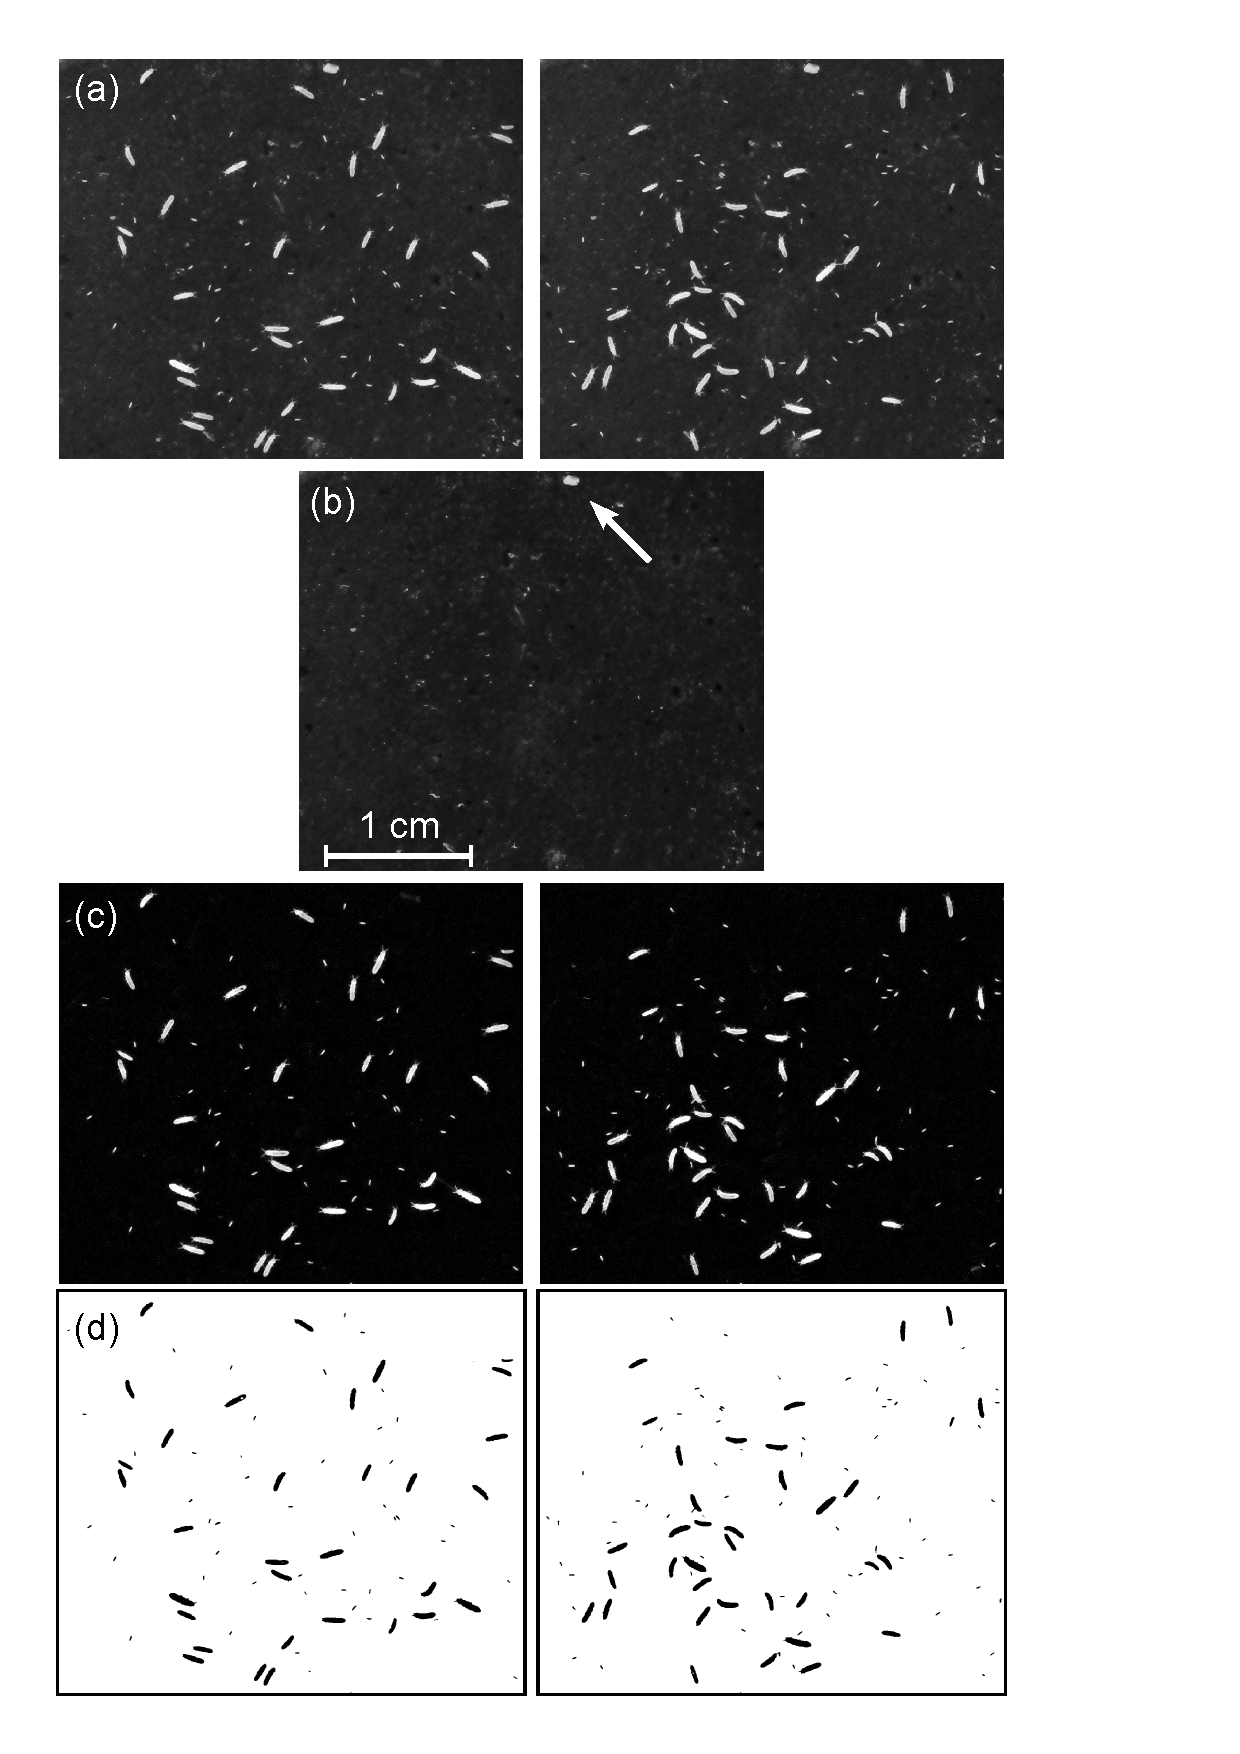
\includegraphics[width=0.55\textwidth]{1_CorpsDeThese/Methodo/1_collemboles_etapes}
\caption[\lofimage{1_CorpsDeThese/Methodo/1_collemboles_etapes} Les étapes
de l'analyse d'image]{Les étapes successives de l'analyse d'image (exemple
d'une population de collemboles).
(a) Deux photos extraites de la série d'images. (b) Le fond de l'image
reconstruit. Chaque pixel est sélectionné comme étant le plus sombre de la
pile d'image. (c) On soustrait le fond (b) à l'image de départ (a) pour
retirer le fond immobile et révéler les éléments mobiles. Le point blanc
(flèche) a été éliminé. (d) Après sélection de la limite d'intensité, on
peut compter et mesurer facilement chacune des particules.}
\label{fig:photoetapes}
\end{center}
\end{figure}



Le principe de base de la méthode développée consiste à comparer des plusieurs
photographies du même microcosmes prises à quelques secondes d'intervalle, en
gardant l'ensemble du dispositif immobile. Cela permet d'obtenir une série
d'image de la même population où seuls les éléments mobiles au cours de la prise
de vue différent entre les images. Généralement, trois à cinq photos sont
suffisantes pour que tous les individus vivants aient été mobiles entre au
moins la première et la dernière photo de la série (Figure
\ref{fig:photoetapes}a).

Au cours de nos expériences, l'ensemble des photos ont été prises avec un
appareil photo réflex piloté par ordinateur (Nikon D300 et
CameraControlPro\textcopyright). Il est également important de disposer d'un
éclairage stable afin que les conditions d'éclairage des prises de vue soient
constantes entre toutes les photos. Nous avons utilisé des ampoules à LED afin
de limiter le risque de fluctuation d'éclairage au cours du temps. 

Une fois la pile d'image obtenue, pour chacune des positions, on sélectionne
dans la pile d'image le pixel le plus sombre à cette position. Les collemboles
étant clairs sur un fond sombre, on reconstruit ainsi une image composite qui
contient uniquement les éléments immobiles au cours de la prise de vue (Figure
\ref{fig:photoetapes}b).
Ainsi, il suffit que tous les pixels de l'image soit au moins une fois sans collembole
dans la série de photos pour que l'image composite représente fidèlement le fond
de la boite. Si un élément clair (une mue par exemple) est présent sur le
substrat, s'il est strictement immobile, il sera également sélectionné comme
fond de l'image (flèche sur la Figure \ref{fig:photoetapes}b). 
On peut alors soustraire le fond immobile de chacune des photos de départ pour
obtenir des images ne contenant que les éléments immobiles (Figure
\ref{fig:photoetapes}c). 

La dernière étape consiste alors à convertir les images en image 8-bits (256
niveaux de gris), et de sélectionner le niveau de gris qui permettra de faire la
différence entre les collemboles et le reste de l'image (limite d'intensité,
Figure \ref{fig:photoetapes}d). Cela crée une image 2-bits (noir ou blanc) sur
la quelle le logiciel ImageJ peut détecter les contours et mesurer les
particules (pour nous les collemboles).

La série d'opération décrite a ensuite été automatisée dans un plugin pour
ImageJ où la plupart des étapes sont automatiques afin de bénéficier d'un
rendement accru dans le traitement des images.

\subsection{Fiabilité de la méthode}

Nous avons testé notre méthode sur différents critères \begin{enumerate*}[label=(\roman*), before=\unskip{ : }, itemjoin={{ ; }},
itemjoin*={{ ; et }}] 
\item le nombre d'image nécessaires au calcul du fond
\item la répétabilité de la mesure de la structure de la population
\item la fiabilité du dénombrement de la population
\end{enumerate*}

\begin{figure}[!ht]
\begin{center}
\includegraphics[width=0.80\textwidth]{1_CorpsDeThese/Methodo/6_Plugin_multiP}
\caption[\lofimage{1_CorpsDeThese/Methodo/6_Plugin_multiP} Analyse de la
fiabilité]{Analyse de la fiabilité de la méthode de mesure. (a) Biosurface
totale de collemboles mesurée ($mm^2$) en fonction du nombre de photos utilisés
pour constituer le fond. (b) Distribution en taille d'une même population de
collemboles mesurée quatre fois indépendemment par deux utilisateurs
différents, la ligne rouge représente un modèle général additif qui ne montre
aucune différence significative entre les photos ou les séries de mesure. (c)
Biosurface en fonction du nombre d'individus (cercles) comptés automatiquement,
les flèches montrent le nombre d'individus comptés à la main, la ligne
pointillée représente une régression linéaire sur les premiers points de mesure.
(d) Comparaison du nombre d'individus comptés automatiquement et à la main. }
\label{fig:photofiabi}
\end{center}
\end{figure}

\subsubsection{Nombre d'image pour le calcul du fond}

Dix populations contenant des densités croissantes d'individus de $0.25$ à
$0.5mm$ ont été prises en photos dans les conditions décrites précédemment avec
des séries de 20 photos. La biosurface d'individus (surface occupée sur la photo
par les individus) a été compté pour chacune des dix populations en utilisant un
nombre croissant d'image pour le calcul du fond. Si la densité d'individus est
élevée dans la populations, un plus grand nombre de photos sont nécessaires pour
obtenir une image fidèle du fond de la boite, dépourvu d'individus mobiles qui
auraient du être éliminés. Bien qu'à faible densité le nombre de photo utilisées
pour le fond de la boite ait peu d'effet sur la mesure de densité, à forte
densité, les mesures répétées dans les populations montrent que la biosurface
mesurée augmente avec le nombre d'image utilisées pour le fabriquer le fond
(Figure ref{fig:photofiabi}a). Il faut un minimum de quatre à cinq images à très
fortes densités pour obtenir une mesure fiable. En revanche il n'est pas
nécessaire d'utiliser plus que six images pour établir le fond, la mesure
de densité n'est pas améliorée. 

\subsubsection{Répétabilité de la mesure de la structure en taille}

Quatres jeux de cinq photos ont été analysés. Deux utilisateurs différents ont
prix chacun deux jeux de photos à quelques minutes d'intervalle pour assurer
l'indépendance des mesures. Les distributions en taille mesurées pour chacun des
quatre jeux de photos sont alors superposés et comparés en utilisant un modèle
additif autorégressif (Figure \ref{fig:photofiabi}b). Les quatre distributions
obtenues se recouvre largement et aucune différence significative n'a pu être
mise en évidence. Notre méthode permet donc une mesure fiable et répétable de la
structure en taille de la population.

\subsubsection{Fiabilité du dénombrement}

Le nombre de particule et leur surface ont été comptés avec la procédure
automatique sur dix populations de densité croissante. Ces mesures automatiques
sur des jeux de vingt photos ont ensuite été comparées à des comptages manuels
du nombre d'individus. 

En dessous de 1000 individus, notre méthode de comptage d'individus présente une
remarquable fiabilité (Figure \ref{fig:photofiabi}d). Au delà de cette densité,
le nombre d'individus comptabilisés par la méthode automatique est de plus en
plus sous-estimé par rapport au comptage manuel. En effet, lorsque la densité
augmente, de plus en plus d'individus se touchent sur les photos et sont alors
détectés comme une seule grosse particule. La biosurface devient alors un
meilleur proxy pour le nombre d'individu à supposer que tous les individus aient
une taille similaire, ce qui est le cas dans cet exemple. On peut alors projeter
la relation entre biosurface et nombre d'individus obtenue à faible densité pour
les forte densité et ainsi connaitre le nombre d'individus en mesurant la
biosurface (Figure \ref{fig:photofiabi}c).

\subsection{En conclusion}

En conclusion, cette méthode présente une grande fiabilité et permet d'accéder à
moindre coût à plusieurs mesures au sein des populations de collemboles pour une
perturbation minimale. Pour cette thèse, cette méthode permet d'accéder au
nombre d'individus ainsi qu'à la longueur corporelle et la biosurface de chacun
des individus, donnant ainsi une mesure de la structure des populations. 

De plus l'implémentation automatisée de la méthode permet de mesurer un grand
nombre de population dans un temps réduit. Une centaine de populations sont
ainsi dénombrées en environ trois heures sur un ordinateur dual-core cadencé à
$2.5GHz$ (à raison de $20$ à $30s$ par jeux de 5 photos).

D'autre part, cette méthode peut également être appliqué à d'autres organismes
ou systèmes expérimentaux. Plusieurs exemples d'utilisation sont décrits en
détail en annexe (voir Chapitre \ref{chap:bpsensor}).

\section{Méthode de représentation graphique}

Notre méthode automatisé d'analyse d'image pour le dénombrement et la mesure de
la structure en taille des populations de collemboles nous permet d'accumuler
rapidement un grand nombre de données. Précisément, à chaque date de mesure nous
disposons pour chacune des populations étudiées le nombre d'individus, et pour
chacun des individus sa taille corporelle ainsi que sa biosurface. Au cours de
nos expérimentations, nous avons été amenés à suivre plusieurs dizaines de
populations durant plusieurs dizaines de semaines.
